\documentclass[12pt,a4paper]{article}
\usepackage{graphicx, booktabs, siunitx, amsmath, geometry, float}
\usepackage{subcaption}
\geometry{margin=2.5cm}
\title{Silicon Wafer Testing: Recombination Lifetime and Iron Contamination Analysis}
\author{Gregorio Jaca (U8L9B9) \and Peter Tallosy (K14WR1)}
\date{\today}

\begin{document}
\maketitle

\begin{abstract}
Charge carrier recombination lifetime is a critical parameter for semiconductor materials, as it quantifiea quality and purity. In this report we look at two main measurements of silicon wafers. First, the concentration of iron (Fe) contamination in a p-type silicon wafer was determined by measuring recombination lifetime before and after the dissociation of iron-boron (Fe-B) pairs. The dynamics of Fe-B pair association were also studied to estimate the iron diffusion constant. Second, the injection-level-dependent recombination lifetime, $\tau(\Delta n)$, was characterized for various silicon wafers and thicker ingots using the eddy-current-based Photoconductance Decay (ePCD) method. Calibration procedures for the measurement system were performed to ensure accuracy in both cases.
\end{abstract}

\section{Introduction}

The efficiency of silicon-based photovoltaic devices is heavily dependent on the recombination lifetime of charge carriers. This parameter provides insight into the material's purity and the presence of defects. Recombination processes, such as Shockley-Read-Hall (SRH), Auger, and radiative recombination, govern the rate at which excess charge carriers return to equilibrium. The total recombination rate is the sum of these individual contributions, and the effective lifetime $\tau_{eff}$ is given by:
\begin{equation}
\frac{1}{\tau_{eff}} = \frac{1}{\tau_{rad}} + \frac{1}{\tau_{Auger}} + \frac{1}{\tau_{SRH}}
\end{equation}
% In addition to bulk recombination, surface recombination at the wafer's interfaces can significantly impact the measured lifetime, especially in thin samples. The overall effective lifetime is a combination of bulk ($\tau_{bulk}$) and surface ($\tau_{surf}$) components:
% \begin{equation}
% \frac{1}{\tau_{eff}} = \frac{1}{\tau_{bulk}} + \frac{1}{\tau_{surf}}
% \end{equation}
In this laboratory exercise we characterize these properties using non-contact methods. The microwave-induced photoconductance decay ($\mu$PCD) technique is used to measure the iron concentration in a p-type silicon wafer. Iron, a common contaminant, forms Fe-B pairs that act as recombination centers. By dissociating these pairs with high-intensity light, the change in lifetime can be used to quantify the iron concentration $N_{Fe}$:
\begin{equation}
N_{Fe} = C_{\mu PCD} \left( \frac{1}{\tau_{before}} - \frac{1}{\tau_{after}} \right)
\end{equation}
where $\tau_{before}$ and $\tau_{after}$ are the lifetimes before and after dissociation, and $C_{\mu PCD}$ is a calibration constant.

The second part of the exercise uses the eddy-current-based PCD (ePCD) method to determine the injection-level-dependent lifetime, $\tau(\Delta n)$, for various samples. While the effective lifetime $\tau_{eff}$ is straightforward to measure from the excitation and decay curves, more sofisticated techniques are required to obtain the $\tau(\Delta n)$, which provides more information about the sample under study, and is particularly important in exotic samples where the recombination lifetime can vary significantly during the decay. This technique is suitable for thicker silicon ingots and allows for the separation of different recombination mechanisms.

\section{Results and Discussion}

\subsection{Iron Contamination Measurement}
The first measurements involved determining the iron concentration in silicon wafers.

We verified the saturation of the lifetime by repeatedly flashing the wafer and measuring the lifetime at a single point until it reached a stable maximum value, as shown in Figure \ref{fig:t2_saturate}. This ensures the complete dissociation of Fe-B pairs into interstitial iron (Fe$_i$) and boron.

\begin{figure}[H]
    \centering
    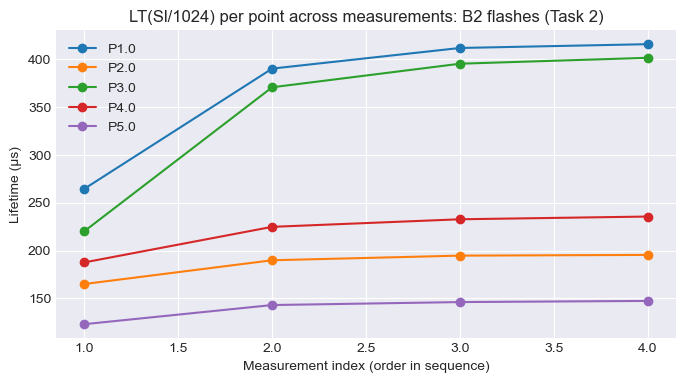
\includegraphics[width=0.5\linewidth]{plots/t2_saturate.png}
    \caption{Lifetime saturation curve showing the increase in charge carrier lifetime as Fe-B pairs are dissociated by high-intensity light flashes.}
    \label{fig:t2_saturate}
\end{figure}

\subsubsection*{Methodology for C and N\textsubscript{Fe} Calculation}

During the laboratory excercise we used the average lifetine value of he whole waffer for our calculations, which gave a significatly smaller value for $C_{\mu PCD}$. This was because the $C_{\mu PCD}$ should be averaged, not the lifetime. To obtain a more robust estimation, a per-point calculation was performed across the entire wafer map for $C_{\mu PCD}$, and then we calculated the mean. This have an even smaller value (more error), with a standard deviation two orders of magnitude larger than the mean value. This suggested that outliers were degrading the data quality, and this was verified by looking at the distribution of lifetimes. To handle outliers in the per-point data, several data cleanup methods were used:
\begin{itemize}
    \item \textbf{Filtering:} Data points were first filtered to ensure physical consistency. Only pixels where the lifetime after dissociation was greater than before ($\tau_{after} > \tau_{before}$) were kept. Additionally, lifetimes were required to be within a plausible range of 20 \si{\micro\second} to 1000 \si{\micro\second} to exclude measurement artifacts.
    \item \textbf{Trimming:} On the filtered dataset, a 1\% trim was applied, removing the lowest and highest 1\% of the calculated $C$ (or $N_{Fe}$) values to further reduce the influence of extreme outliers.
\end{itemize}

This cleanup removed less than 5\% of total data points, so we consider it reasonable. The uncertainty of the central tendency (mean and median) was assessed using two methods:
\begin{itemize}
    \item \textbf{Standard Error (SE):} The standard error of the mean was calculated as $SE_{mean} = \sigma / \sqrt{n}$, where $\sigma$ is the sample standard deviation. For the median: $SE_{med} \approx 1.2533 \times MAD / \sqrt{n}$, where MAD is the Median Absolute Deviation.
    \item \textbf{Bootstrap Half-Width (95\% CI):} The data was resampled with replacement 10,000 times, and the mean or median was calculated for each sample. The 2.5th and 97.5th percentiles of the resulting distribution defined the confidence interval. The error half-width is reported as $(upper - lower)/2$.
\end{itemize}

The results of this analysis for both $C_{\mu PCD}$ and $N_{Fe}$ are presented in Table \ref{tab:C_results} and Table \ref{tab:NFe_results}, respectively. The median-based methods, particularly after filtering and trimming, provided the most stable estimates with the smallest errors.

\begin{table}[H]
    \centering
    \caption{Statistical analysis of the iron constant $C_{\mu PCD}$ using different calculation methods.}
    \label{tab:C_results}
    \begin{tabular}{@{}lS[table-format=1.4e2]S[table-format=4.0]S[table-format=1.4e2]S[table-format=1.4e2]@{}}
        \toprule
        Method         & {Value (cm$^3\cdot\mu$s)} & {Count} & {SE} & {Bootstrap HW (95\% CI)} \\
        \midrule
        Raw Mean       & 2.8406e13 & 4328 & 4.1625e13 & 6.7624e13 \\
        Raw Median     & 7.0258e13 & 4328 & 3.6318e11 & 9.7242e11 \\
        Filtered Mean  & 7.6493e13 & 4165 & 4.0648e12 & 7.5349e12 \\
        Filtered Median& 7.1458e13 & 4165 & 3.4511e11 & 9.4144e11 \\
        Trimmed Mean   & 6.8337e13 & 4081 & 4.9012e11 & 9.5759e11 \\
        Trimmed Median & 7.1458e13 & 4081 & 3.3788e11 & 9.5443e11 \\
        \bottomrule
    \end{tabular}
\end{table}

Using the trimmed median value for $C$ ($7.15 \times 10^{13}$ cm$^3\cdot\mu$s), we calculated the iron concentration $N_{Fe}$ of the sample. The results are shown in Table \ref{tab:NFe_results}. The filtered and trimmed median values are consistent, giving $N_{Fe} \approx 2.81 \times 10^{10}$ cm$^{-3}$.

\begin{table}[H]
    \centering
    \caption{Statistical analysis of the iron concentration $N_{Fe}$ (cm$^{-3}$).}
    \label{tab:NFe_results}
    \begin{tabular}{@{}lS[table-format=1.4e2]S[table-format=4.0]S[table-format=1.4e2]S[table-format=1.4e2]@{}}
        \toprule
        Method         & {Value (cm$^{-3}$)} & {Count} & {SE} & {Bootstrap HW (95\% CI)} \\
        \midrule
        Raw Mean       & 6.0515e10 & 4294 & 3.8284e9 & 7.4921e9 \\
        Raw Median     & 1.7808e10 & 4294 & 3.7997e8 & 1.2023e9 \\
        Filtered Mean  & 8.2129e10 & 2906 & 3.7834e9 & 7.4527e9 \\
        Filtered Median& 2.8123e10 & 2906 & 2.7525e8 & 6.6961e8 \\
        Trimmed Mean   & 6.8405e10 & 2846 & 2.7232e9 & 5.3240e9 \\
        Trimmed Median & 2.8123e10 & 2846 & 2.7014e8 & 6.6682e8 \\
        \bottomrule
    \end{tabular}
\end{table}

This method and values were employed in the following sections.

\subsection{Investigation of Fe-B Association Kinetics}
We monitored the re-association of Fe-B pairs over time by performing lifetime mappings at 10-minute intervals after the initial dissociation. The concentrations of dissociated iron ($Fe_i$) was calculated at each time step. The results, averaged over five measurement points, are plotted in Figure \ref{fig:task5} \footnote{For this task we re-calculated the value for $C$ to make sure we would get similar results using just 5 data points, as compared to doing it with the whole sample. We obtained very similar results.}.

\begin{figure}[H]
    \centering
    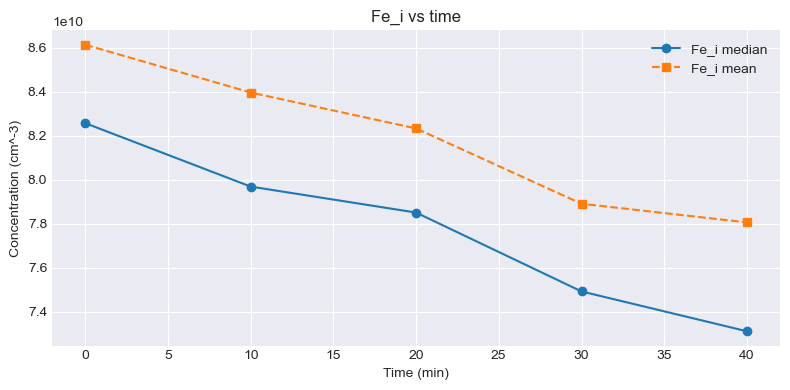
\includegraphics[width=0.6\linewidth]{plots/task5.png}
    \caption{Association kinetics of Fe-B pairs. The concentration of interstitial iron ($Fe_i$) decreases over time as it re-associates with boron to form Fe-B pairs.}
    \label{fig:task5}
\end{figure}

The association process is expected to follow first-order kinetics. By fitting an exponential decay to the $Fe_i(t)$ data, we determined the association rate constant $R$. The fit yielded $R = 3.047 \times 10^{-3}$ min$^{-1}$ ($5.078 \times 10^{-5}$ s$^{-1}$) with an $R^2$ value of 0.9822 \footnote{The time constant of the recombination process can be several hours or days, depending on the boron concentration. Having just 5 data points, with a 10 minute interval between measurements }. The iron diffusion constant $D_0$ can be calculated from $R$ using the equation:
\begin{equation}
R = \frac{e^2}{\epsilon \epsilon_0 k_B T} N_B D_0 \exp\left( \frac{-E_{mig}}{k_B T} \right)
\end{equation}

We could not obtain the boron concentration $N_B$, which is necessary for the $D_0$ calculation, so we calculated $D_0$ for a range of reasonable $N_B$ values, as shown in Table \ref{tab:D0_values} \footnote{Here we are unsure if we should have obtained the value from a datasheet or calculated $N_B$ from the conductance of the sample, but we did not have the necessary data to do it}. The calculated $D_0$ values are several orders of magnitude higher than literature values (e.g., $\sim 10^{-14}$ cm$^2$/s), suggesting that we made a mistake in the process.

\begin{table}[H]
    \centering
    \caption{Calculated iron diffusion constant $D_0$ for different assumed boron concentrations $N_B$.}
    \label{tab:D0_values}
    \begin{tabular}{@{}S[table-format=1.2e2]S[table-format=1.4e-4]@{}}
        \toprule
        {$N_B$ (cm$^{-3}$)} & {$D_0$ (cm$^2$/s)} \\
        \midrule
        1.00e15 & 4.79e-4 \\
        3.00e15 & 1.60e-4 \\
        1.00e16 & 4.80e-5 \\
        3.00e16 & 1.60e-5 \\
        1.00e17 & 5.00e-6 \\
        \bottomrule
    \end{tabular}
\end{table}

\subsection{ePCD System Calibration}

In the following section we employ the ePCD technique using the WT-1200I device. Accurate ePCD measurements require calibration. We established the relationship between the measured eddy-current signal voltage ($V_{eddy}$) and the sheet conductance ($\sigma_{sh}$) using a set of calibration wafers with known resistivity. A linear fit to the data (Figure \ref{fig:task6}) yielded a slope of 0.8375 S/V and an offset voltage of 1.2123 V, with a high coefficient of determination ($R^2 = 0.9985$). We also measured the DC level for the voltage, 1.225V, and we tried to use that, but we obtained much better results using the voltage offset calculated from the linear fit, 1.2123V, which is still close to the other value.

\begin{figure}[H]
    \centering
    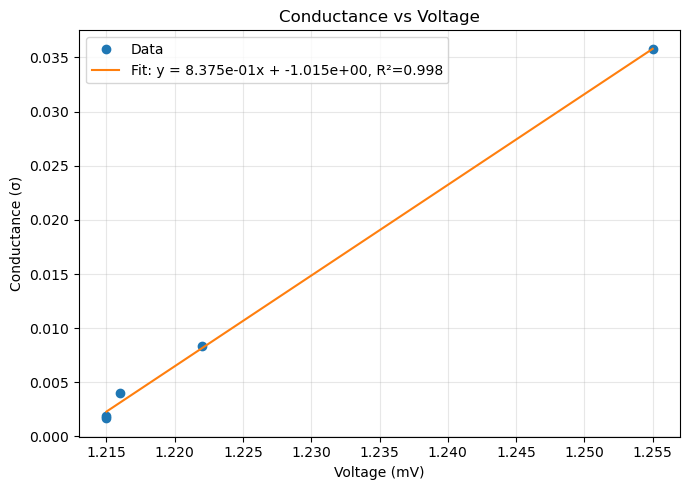
\includegraphics[width=0.6\linewidth]{plots/task6.png}
    \caption{Calibration curve for sheet conductance ($\sigma_{sh}$) vs. eddy-current voltage ($V_{eddy}$). The data is fitted with a linear function to determine the system's response.}
    \label{fig:task6}
\end{figure}

We investigated the system's sensitivity depth using thick silicon slugs. The apparent sheet conductance was used to calculate a sensitivity depth $d_{sense}$. A linear relationship was found between $V_{eddy}$ and $d_{sense}$ (Figure \ref{fig:task7_fit}), with $R^2 = 0.9986$ after excluding two initial data points that did not follow the trend \footnote{Honestly we do not know why.}. % GGG
%This calibration is crucial for interpreting measurements on thick samples where the signal originates from a volume rather than a thin sheet.

\begin{figure}[H]
    \centering
    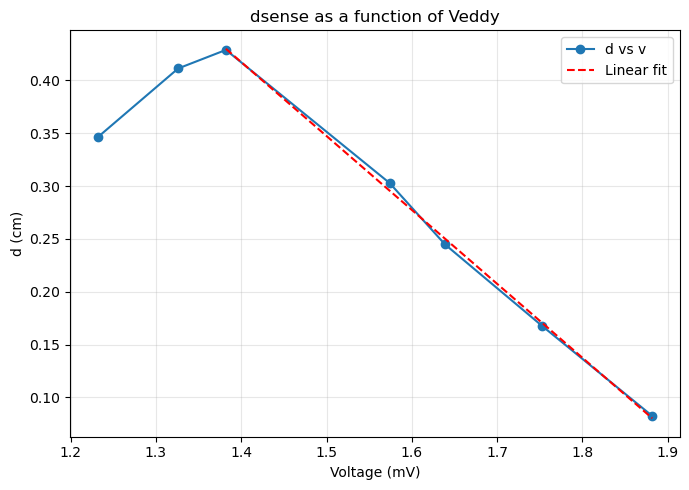
\includegraphics[width=0.6\linewidth]{plots/task7_fit.png}
    \caption{Calibration curve for sensitivity depth ($d_{sense}$) vs. eddy-current voltage ($V_{eddy}$) for thick silicon slugs.}
    \label{fig:task7_fit}
\end{figure}

\subsection{Injection-Dependent Lifetime on Wafers}
The WT-1200I device calculates the $\tau_{eff}$ for each excitation. We measured the injection-dependent lifetime $\tau(\Delta n)$ on two different n-type solar cell wafers. A key step in this analysis is the accurate determination of the excess carrier concentration, $\Delta n$, from the measured sheet conductance, $\sigma_s$ (The relationship between the conductance and $V_{eddy}$ was previously determined and is used here). This requires accounting for the dependence of carrier mobility on both dopant concentration ($N_{dop}$) and the injection level ($\Delta n$) itself. The relationship is given by:
\begin{equation}
\Delta n = \frac{\sigma_s/W - N_{dop}\cdot e \cdot \mu_{maj}(N_{dop}, \Delta n)}{e \cdot \mu_{sum}(N_{dop}, \Delta n)}
\end{equation}
where $W$ is the wafer thickness, $e$ is the elementary charge, and $\mu_{maj}$ and $\mu_{sum}$ are the majority carrier and summed mobilities, respectively. To solve this implicit equation for $\Delta n$, an iterative method was employed. The calculation started with an initial guess for $\Delta n$ to calculate the mobilities, then a new $\Delta n$ was computed. This process was repeated until the value of $\Delta n$ converged within a tolerance of $10^{-3}$ cm$^{-3}$. The tolerance is several orders of magnitude smaller than the value for $\Delta n$. The mobility values were obtained from a validated calculator based on the model provided by PV Lighthouse \footnote{We reverse engineered the calculator and validated that we obtained the same outputs for the same inputs and then we used it in the code.}.

Once the $\Delta n(t)$ decay curve was obtained, the lifetime $\tau(\Delta n)$ was calculated using the transient formula $\tau(\Delta n) = - \Delta n / (\partial\Delta n/\partial t)$. The numerical differentiation of the noisy experimental data was performed using a Savitzky-Golay filter with a third-order polynomial and a window length of 21 points (corresponding to a time window of 420 ns), which was found to provide optimal smoothing without distorting the underlying signal \footnote{This assessment was qualitative but we did visually inspect every curve to make sure that the differentiation looked reasonable.}.

\begin{figure}[H]
    \centering
    \begin{subfigure}[b]{0.48\linewidth}
        \centering
        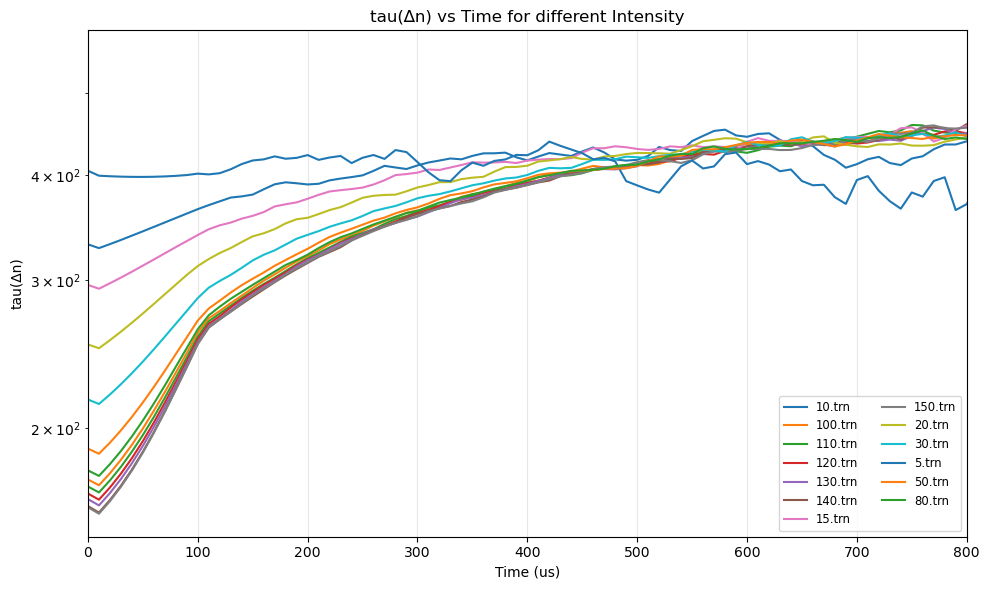
\includegraphics[width=\linewidth]{plots/tau_t_second_different_intensity.png}
        \caption{Sample kx64-b1-449, $\tau(t)$}
    \end{subfigure}\hfill
    \begin{subfigure}[b]{0.48\linewidth}
        \centering
        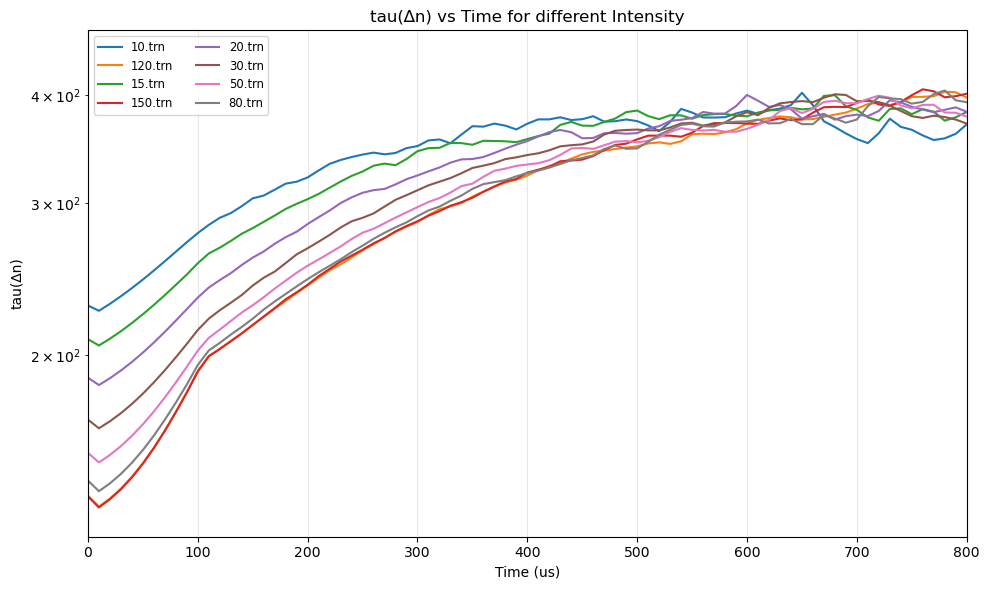
\includegraphics[width=\linewidth]{plots/tau_t_third_different_intensity.png}
        \caption{Sample kx64-b1-615, $\tau(t)$}
    \end{subfigure}
    \begin{subfigure}[b]{0.48\linewidth}
        \centering
        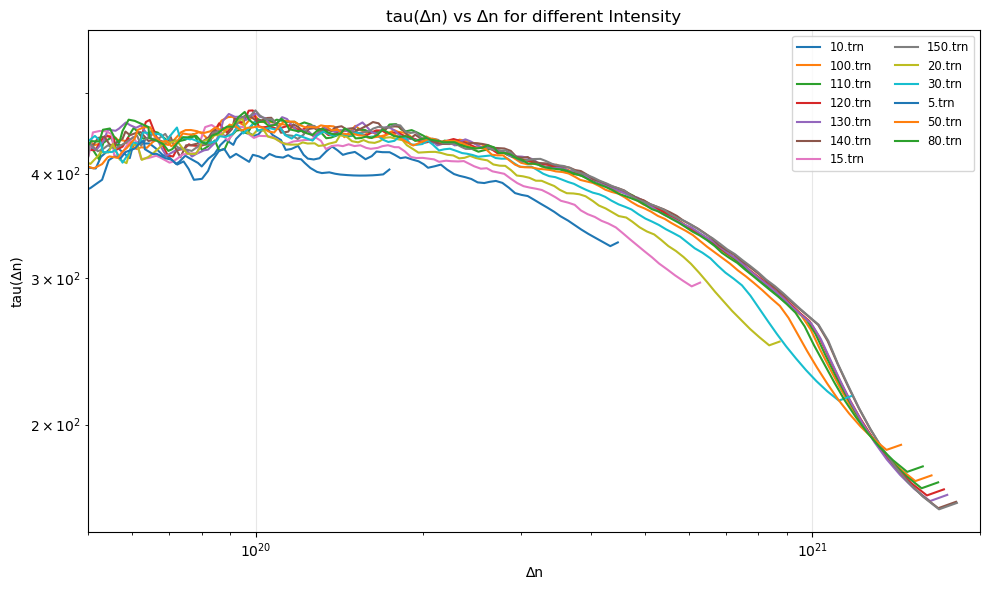
\includegraphics[width=\linewidth]{plots/tau_dn_second_different_intensity.png}
        \caption{Sample kx64-b1-449, $\tau(\Delta n)$}
    \end{subfigure}\hfill
    \begin{subfigure}[b]{0.48\linewidth}
        \centering
        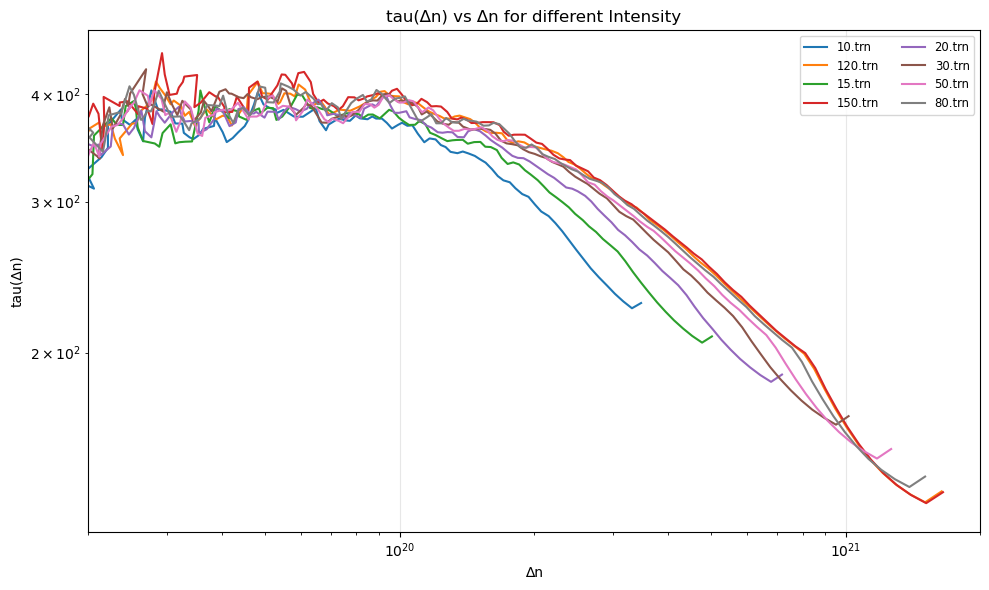
\includegraphics[width=\linewidth]{plots/tau_dn_third_different_intensity.png}
        \caption{Sample kx64-b1-615, $\tau(\Delta n)$}
    \end{subfigure}
    \caption{Recombination lifetime for two passivated wafers (kx64-b1-449 and kx64-b1-615) measured at different laser intensities. The top plots show lifetime vs. time, and the bottom plots show lifetime vs. injection level.}
    \label{fig:wafers_intensity}
\end{figure}

Figure \ref{fig:wafers_intensity} shows the results for two passivated wafers measured at different laser intensities. The top row shows the lifetime as a function of time, while the bottom row shows the lifetime as a function of injection level. The curves show that lifetime is strongly dependent on the injection level, with orders of magnitude changes in its value during decay. The different laser powers result in different maximum injection levels, but the underlying $\tau(\Delta n)$ curves overlap, showing their similar dynamics. On top of that, most. In Figure \ref{fig:wafers_intensity} (a) we can clearly see that for low intensity excitations, $\tau$ is constant with respect to time. This is because the electron-hole pairs are very few and this does not saturate, making this cases unsuitable for measurement.

\subsection{Injection-Dependent Lifetime on Ingots}
The investigation was extended to unpassivated silicon ingots (samples kx77 and kx78) of varying thickness. For these samples, surface recombination is expected to be a stronger factor. We measured the decay curves at different laser intensities and sample widths.

Figure \ref{fig:ingots_dn_t} shows the raw decay of the excess carrier density $\Delta n(t)$ for the thickest ingot from each set (kx77 and kx78) under varying laser intensity, and also using the maximum intensity but for different thickness or width. Figure \ref{fig:ingots_dn_t} (c) shows very well the dependance on the laser intensity, although, above an intensity of 50E11, the curves were similar. Below that intensity, the electron-hole pair creation does not saturate, which could also be observed in the excitation curves.

\begin{figure}[H]
    \centering
    \begin{subfigure}[b]{0.48\linewidth}
        \centering
        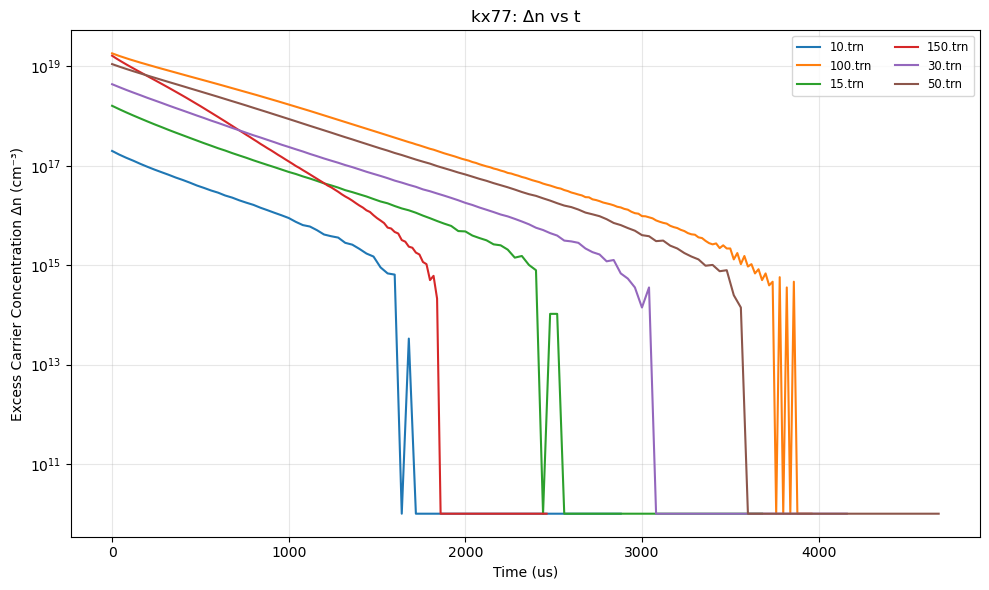
\includegraphics[width=\linewidth]{plots/dn_t_kx77_first_different_intensity.png}
        \caption{kx77, varying intensity}
    \end{subfigure}\hfill
    \begin{subfigure}[b]{0.48\linewidth}
        \centering
        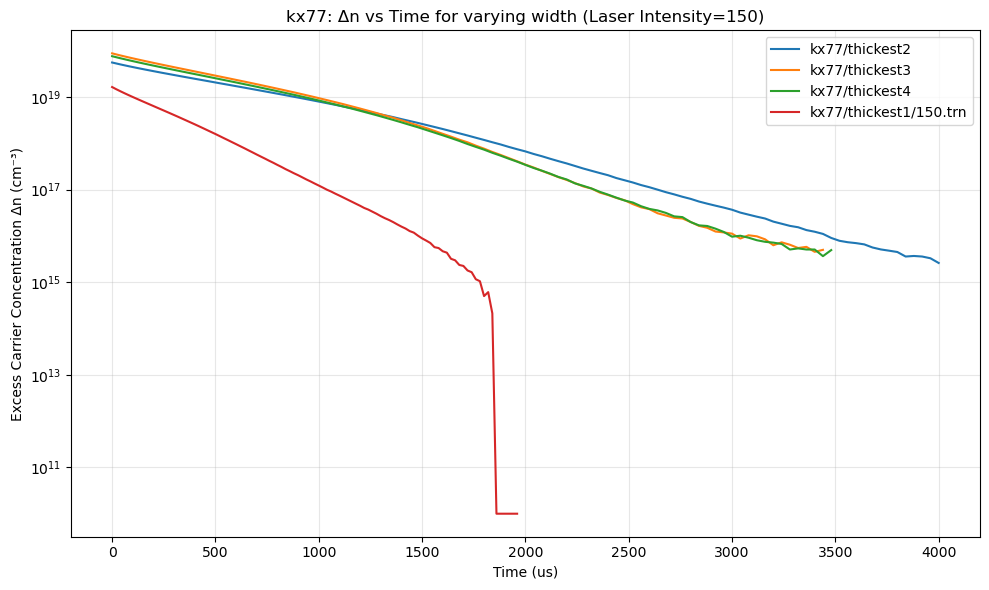
\includegraphics[width=\linewidth]{plots/dn_t_kx77_first_different_width.png}
        \caption{kx77, varying sample width}
    \end{subfigure}
    \begin{subfigure}[b]{0.48\linewidth}
        \centering
        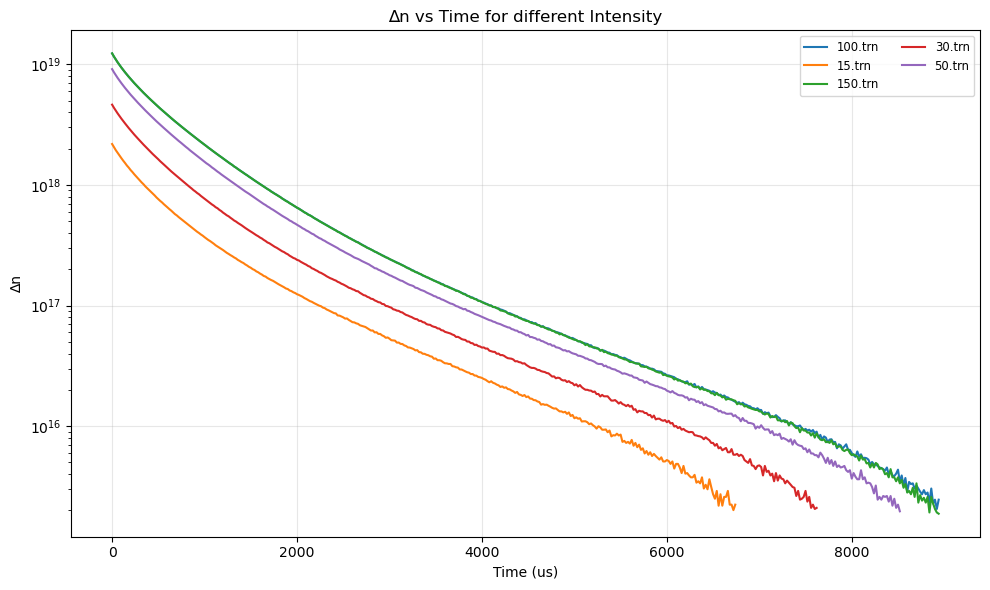
\includegraphics[width=\linewidth]{plots/dn_t_kx78_first_different_intensity.png}
        \caption{kx78, varying intensity}
    \end{subfigure}\hfill
    \begin{subfigure}[b]{0.48\linewidth}
        \centering
        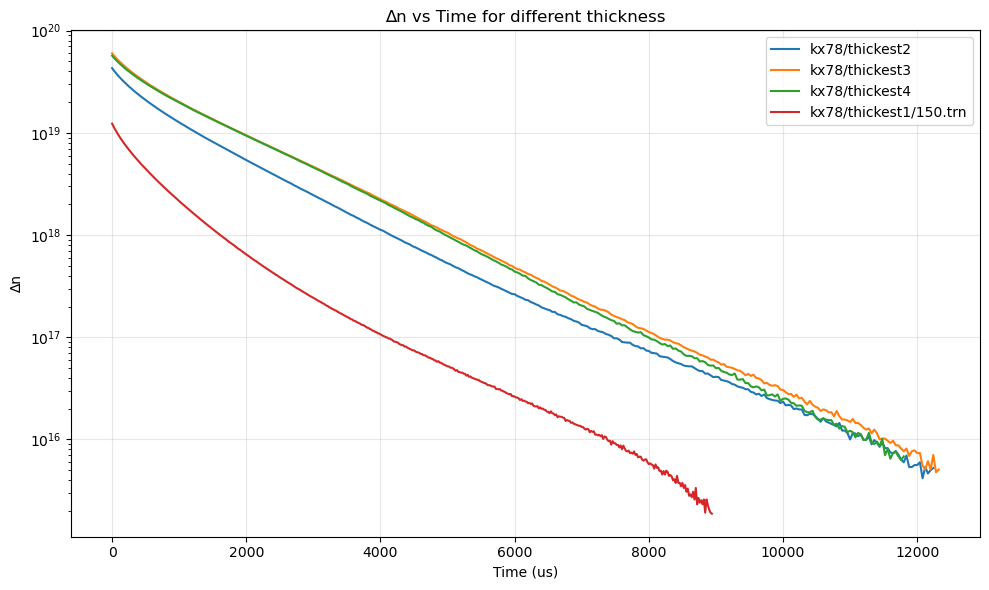
\includegraphics[width=\linewidth]{plots/dn_t_kx78_first_different_width.png}
        \caption{kx78, varying sample width}
    \end{subfigure}
    \caption{Excess carrier density decay $\Delta n(t)$ for the thickest ingots from sets kx77 and kx78, measured with different laser intensities and sample widths.}
    \label{fig:ingots_dn_t}
\end{figure}



The corresponding $\tau(\Delta n)$ curves for the kx78 ingot are shown in Figure \ref{fig:ingots_tau_dn_k78}. Many clear results can be observed here. Firstly, a strong dependance of $\tau(\Delta n)$ as a function of $\Delta n$. Secondly, we see that stronger light intensities induce higher maximum $\Delta n$ (trivial), but also higher $tau$ even for the same $\Delta n$ (not trivial). Figure \ref{fig:wafers_intensity} (c) and (d) show the same effect.

Lastly, in this case we see that thicker wafers have a lower $tau$ for a given $\Delta n$. We were expecting the opposite for unpassivated samples, since in thinner samples, surface recombination is expected to dominate, which would suggest lower $tau$. We can see singificantly higher $\tau(\Delta n)$ values for the sample kx78 compared to the passivated wafers (Figure \ref{fig:wafers_intensity}). This is not what we expected. Passivated samples are expected to have higher measured lifetime: surface recombination is suppressed, so $\tau_{eff}$ approaches $\tau_{bulk}$. Unpassivated surfaces add a 1/$\tau_{surf}$ term that shortens $\tau_{eff}$. Now, if we look at \ref{fig:ingots_tau_t} (a) and (b) we also see the lifetimes for kx77, which are smaller than those of the passivated samples. So it seems that kx78 is somewhat of an outlier, having such a high lifetime. We also looked at the raw $\tau_{eff}$, which confirm the same picture\footnote{Unfortunately we do not know enough about the kx78 sample to give an explanation for this. We do know that it has a significantly higher doping level, but we could not explain the mechanism behind this difference.}.

\begin{figure}[H]
    \centering
    \begin{subfigure}[b]{0.48\linewidth}
        \centering
        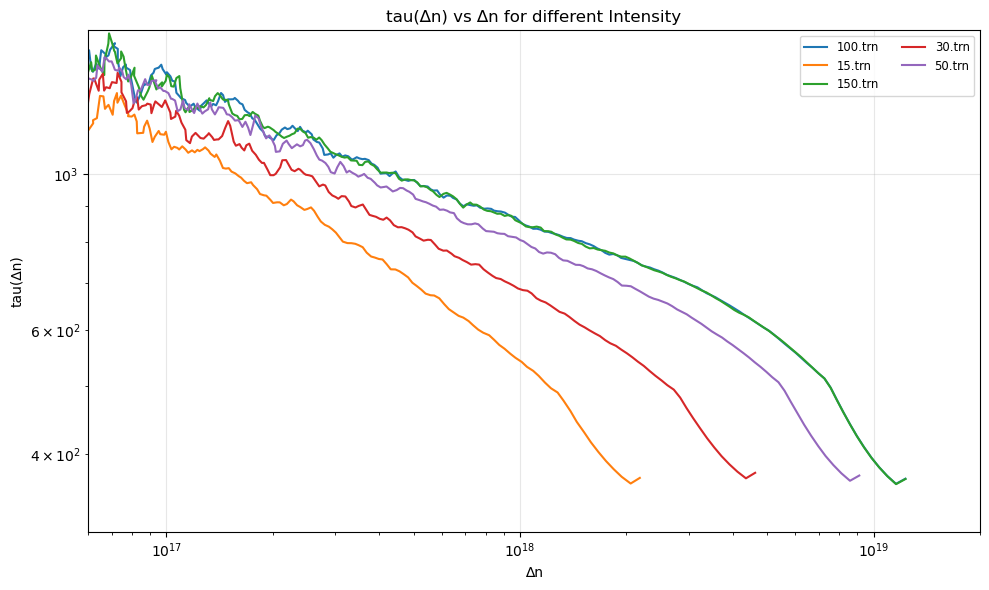
\includegraphics[width=\linewidth]{plots/tau_dn_k78_different_intensity.png}
        \caption{Varying intensity}
    \end{subfigure}\hfill
    \begin{subfigure}[b]{0.48\linewidth}
        \centering
        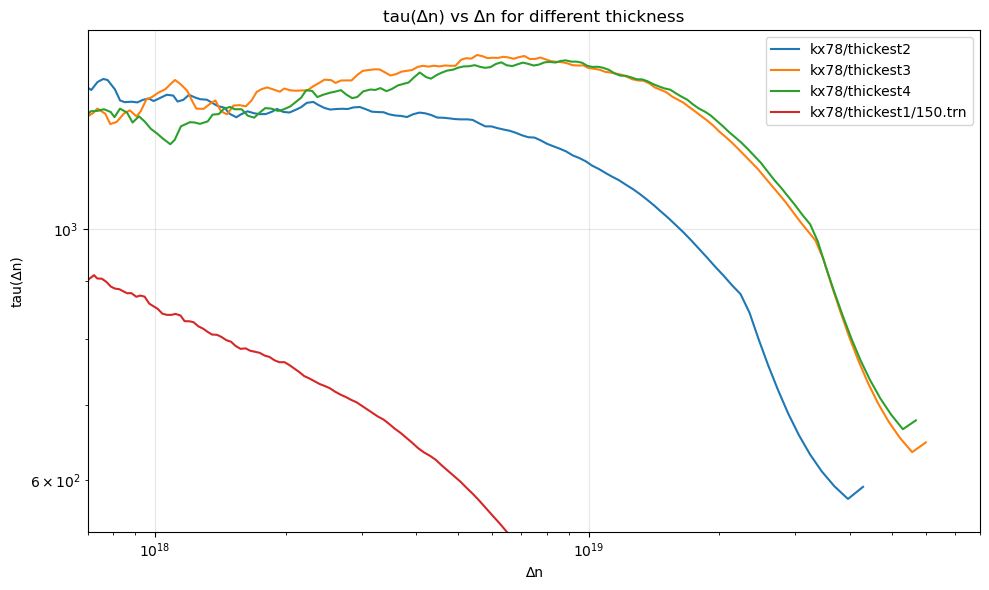
\includegraphics[width=\linewidth]{plots/tau_dn_k78_different_width.png}
        \caption{Varying sample width}
    \end{subfigure}
    \caption{Injection-dependent lifetime $\tau(\Delta n)$ for the kx78 ingot, derived from measurements with varying laser intensity and sample width.}
    \label{fig:ingots_tau_dn_k78}
\end{figure}

Finally, Figure \ref{fig:ingots_tau_t} compares the lifetime evolution over time for the different ingots and measurement conditions. 
% The strong dependence on sample properties and excitation conditions is evident. For unpassivated samples, the measured effective lifetime is dominated by surface effects and diffusion, masking the true bulk lifetime.

\begin{figure}[H]
    \centering
    \begin{subfigure}[b]{0.48\linewidth}
        \centering
        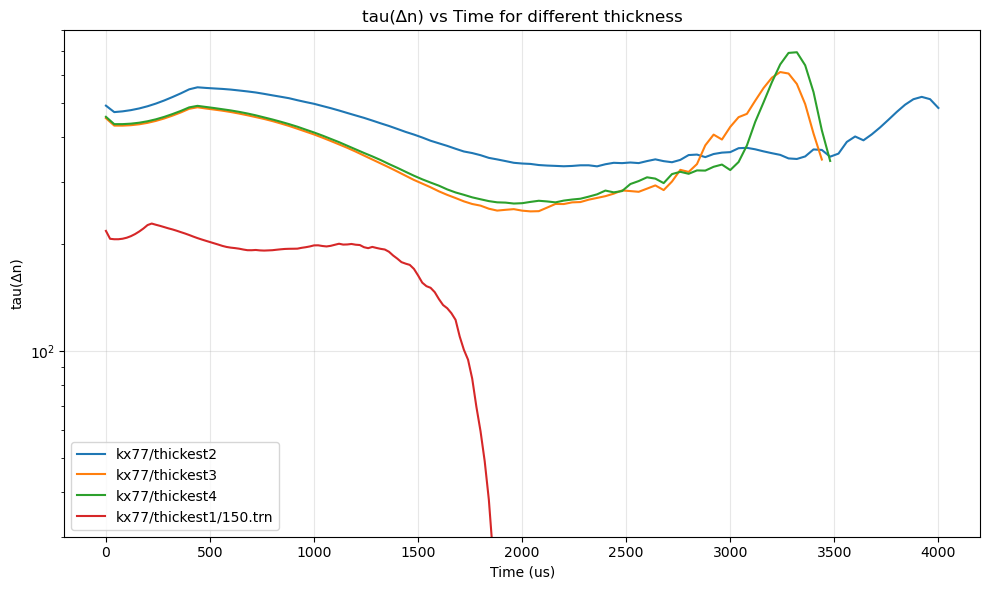
\includegraphics[width=\linewidth]{plots/tau_t_kx77_different_width.png}
        \caption{kx77, varying width}
    \end{subfigure}\hfill
    \begin{subfigure}[b]{0.48\linewidth}
        \centering
        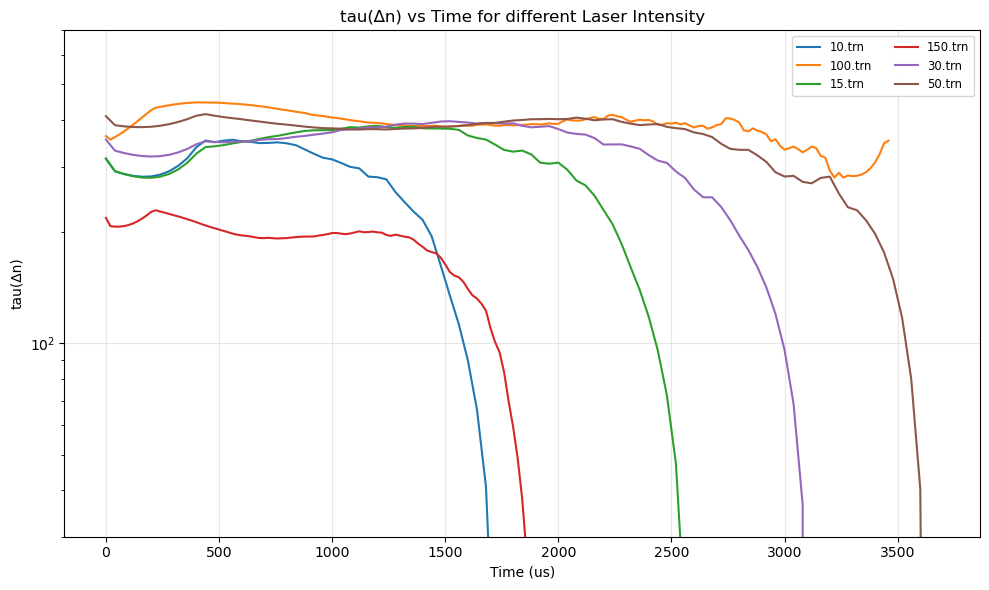
\includegraphics[width=\linewidth]{plots/tau_t_kx77_first_different_intensity.png}
        \caption{kx77, varying intensity}
    \end{subfigure}
    \begin{subfigure}[b]{0.48\linewidth}
        \centering
        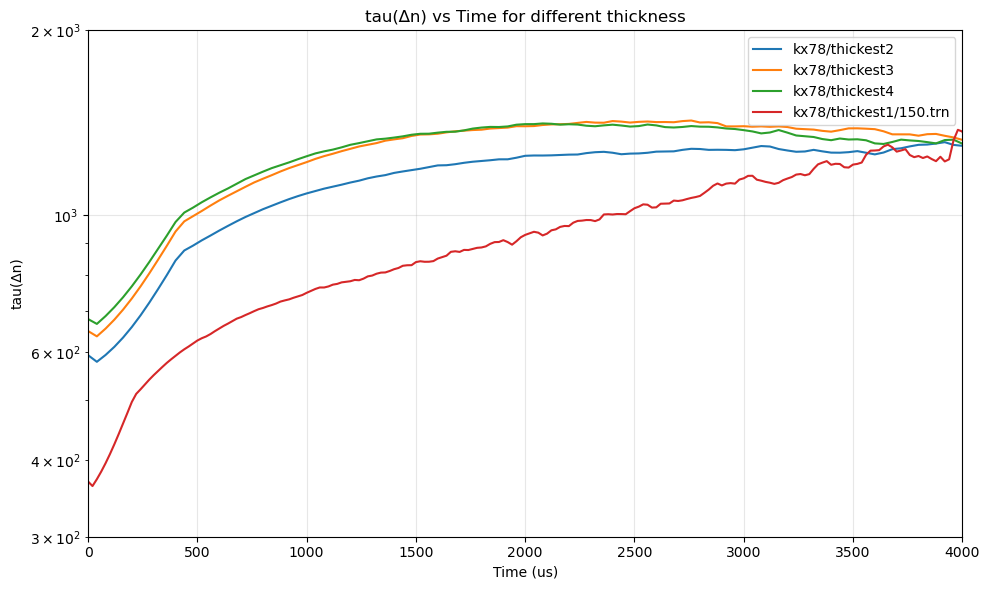
\includegraphics[width=\linewidth]{plots/tau_t_kx78_different_width.png}
        \caption{kx78, varying width}
    \end{subfigure}\hfill
    \begin{subfigure}[b]{0.48\linewidth}
        \centering
        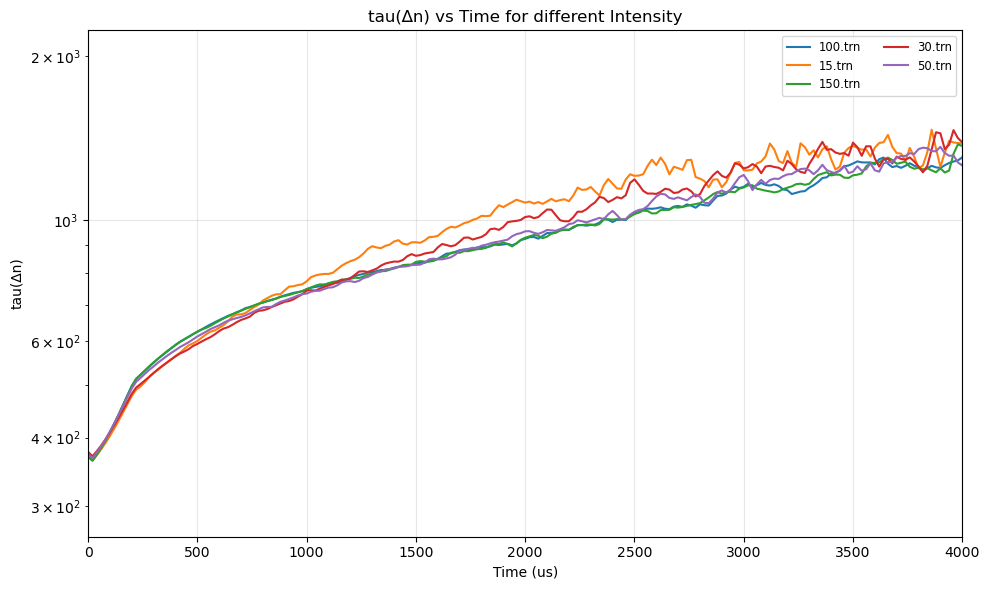
\includegraphics[width=\linewidth]{plots/tau_t_kx78_first_different_intensity.png}
        \caption{kx78, varying intensity}
    \end{subfigure}
    \caption{Lifetime vs. time, $\tau(t)$, for the kx77 and kx78 ingots under different measurement conditions.}
    \label{fig:ingots_tau_t}
\end{figure}


\subsection{Separation of Bulk and Surface Lifetime Components}

The measured effective carrier lifetime ($\tau_{eff}$) in a silicon sample is determined by:

\begin{equation}
    \frac{1}{\tau_{eff}(\Delta n)} = \frac{1}{\tau_{bulk}(\Delta n)} + \frac{1}{\tau_{surface}(\Delta n)}
    \label{eq:tau_{eff}_separation}
\end{equation}

For unpassivated silicon ingots with high surface recombination velocities:
% GGG

\begin{equation}
    \tau_{surface} \approx \frac{W^2}{\pi^2 D}
    \label{eq:tau_surf_diffusion}
\end{equation}

\begin{equation}
    \frac{1}{\tau_{eff}} = \frac{1}{\tau_{bulk}} + \left(\pi^2 D\right) \cdot \frac{1}{W^2}
    \label{eq:linear_fit_model}
\end{equation}

To separate the components, measurements of $\tau_{eff}$ were performed on the same ingot at varying thicknesses ($W$). For each injection level $\Delta n$, a linear regression was performed plotting $1/\tau_{eff}$ versus $1/W^2$. The bulk component was extracted from the fit parameters.

\begin{figure}[H]
    \centering
    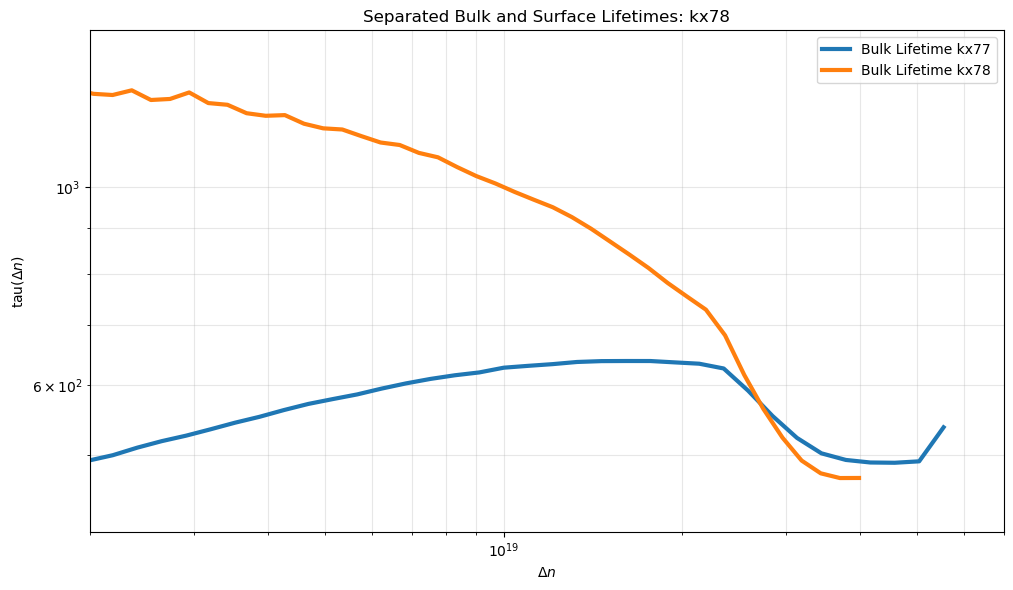
\includegraphics[width=0.6\linewidth]{plots/bulk4.png}
    \caption{$\tau_{bulk}$ for the two samples kx77 and kx78.}
    \label{fig:bulk}
\end{figure}

This method assumes that $\tau_{bulk}$ and the diffusion coefficient $D$ are uniform throughout the ingot and independent of the thickness cut.

\section{Conclusion}
In this laboratory exercise, we successfully characterized key recombination properties of various silicon samples. We determined the iron concentration in a p-type wafer using the $\mu$PCD technique, employing robust statistical methods to derive a reliable calibration constant and reduce the effect of measurement outliers. The study of Fe-B association kinetics allowed for an estimation of the iron diffusion constant, although the final result deviated from the expected value, suggesting some error in our procedure.

The ePCD measurements provided detailed insight into the injection-level-dependent lifetime, $\tau(\Delta n)$. The measurements revealed a strong dependance between $tau$ and $\Delta n$. The consistency of the $\tau(\Delta n)$ curves under different excitation conditions validated the measurement and analysis methodology, but it also showed the need for sufficiently high intensity excitations. Finally we studied the dependance on the sample's thickness, on the type of surface, passivated or unpassivated, and identified $\tau_{bulk}$ and $\tau_{surf}$.

\end{document}
